\hypertarget{_parser_8cpp}{}\section{Visual\+Impro/\+Parser.cpp File Reference}
\label{_parser_8cpp}\index{Visual\+Impro/\+Parser.\+cpp@{Visual\+Impro/\+Parser.\+cpp}}


\mbox{\hyperlink{class_parser}{Parser}} object used to get information from config file.  


{\ttfamily \#include \char`\"{}Parser.\+hpp\char`\"{}}\newline
Include dependency graph for Parser.\+cpp\+:
\nopagebreak
\begin{figure}[H]
\begin{center}
\leavevmode
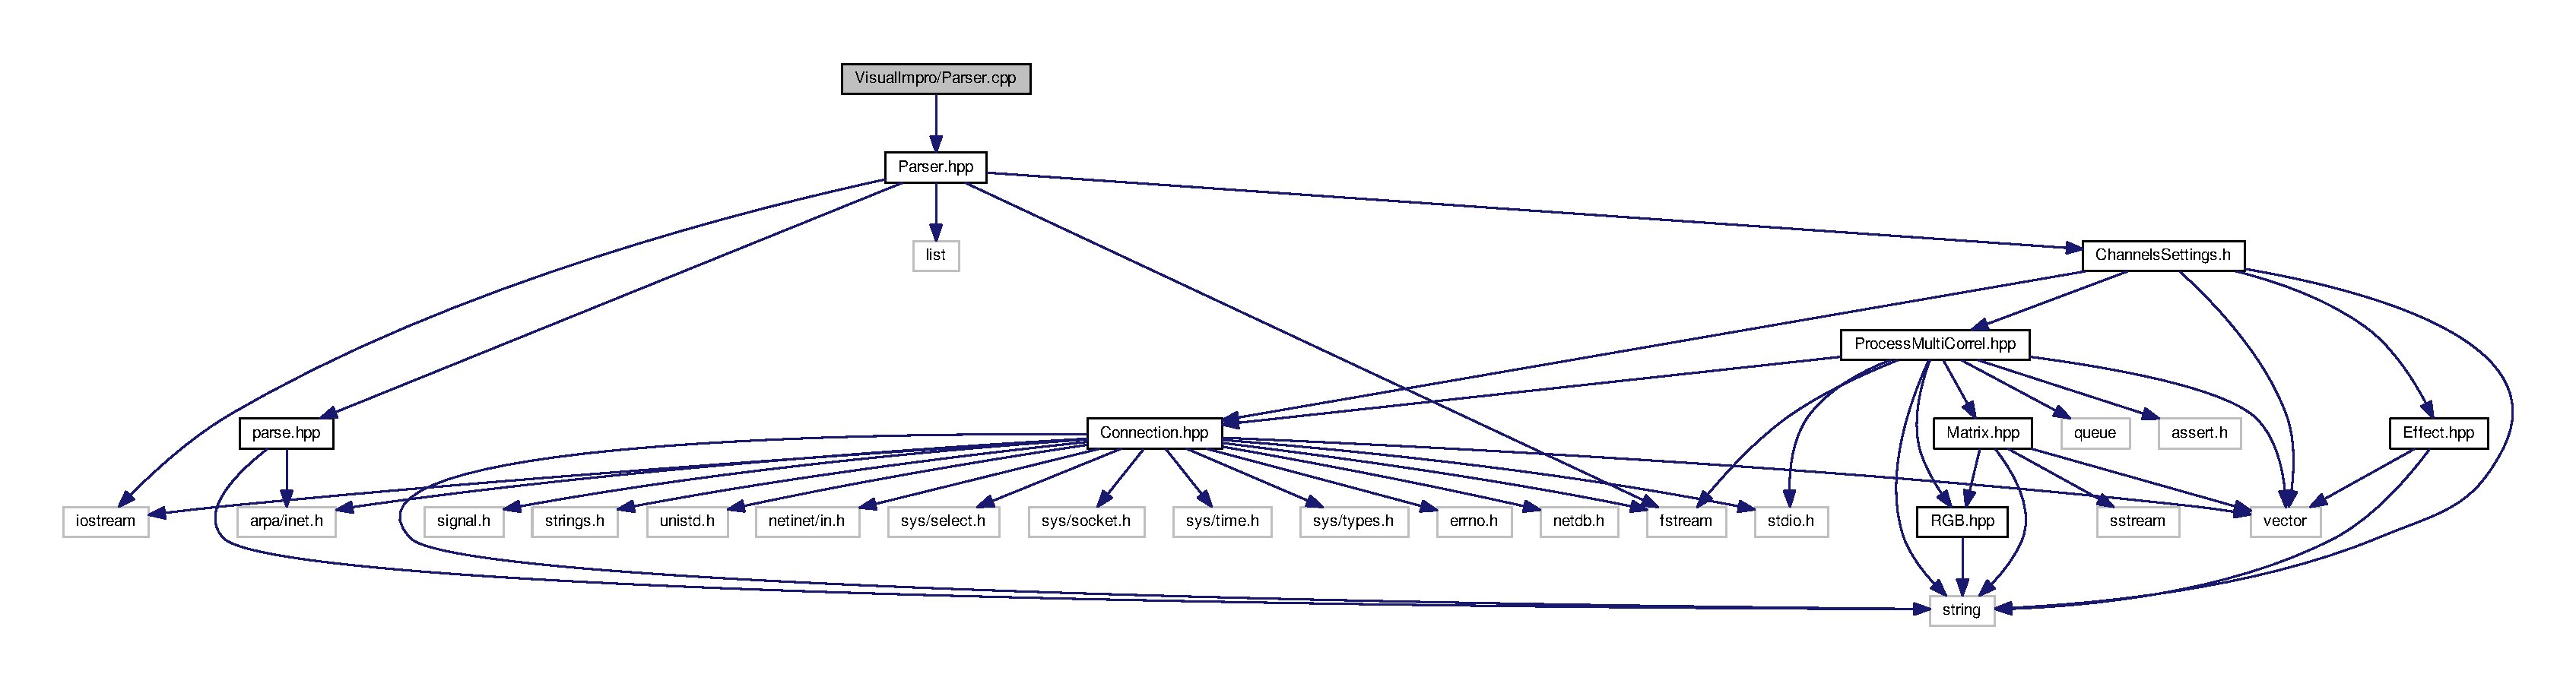
\includegraphics[width=350pt]{_parser_8cpp__incl}
\end{center}
\end{figure}


\subsection{Detailed Description}
\mbox{\hyperlink{class_parser}{Parser}} object used to get information from config file. 

\begin{DoxyAuthor}{Author}
Jérémy L\+I\+X\+A\+N\+D\+RE 
\end{DoxyAuthor}
\begin{DoxyDate}{Date}
July 2017
\end{DoxyDate}
Parses a config file with filenames and functions. It is used in main.\+cpp to fill a Channel settings structure with the parameters given to the program. It is also used to prevent the use of too many occurencies of each element (ex\+: 2 lines with C\+O\+L\+OR). In this case, the last line is kept. 